
\section{Das zentrale Dogma der Molekularbiologie}

\begin{center}
    ``The central dogma states that information in nucleic acid can be perpetuated or transferred, but the transfer of
    information into protein is irreversible''
\end{center}

\begin{center}
    ``DNA macht RNA macht Protein''
\end{center}

\defin{dogma}

\begin{figure}[H]
    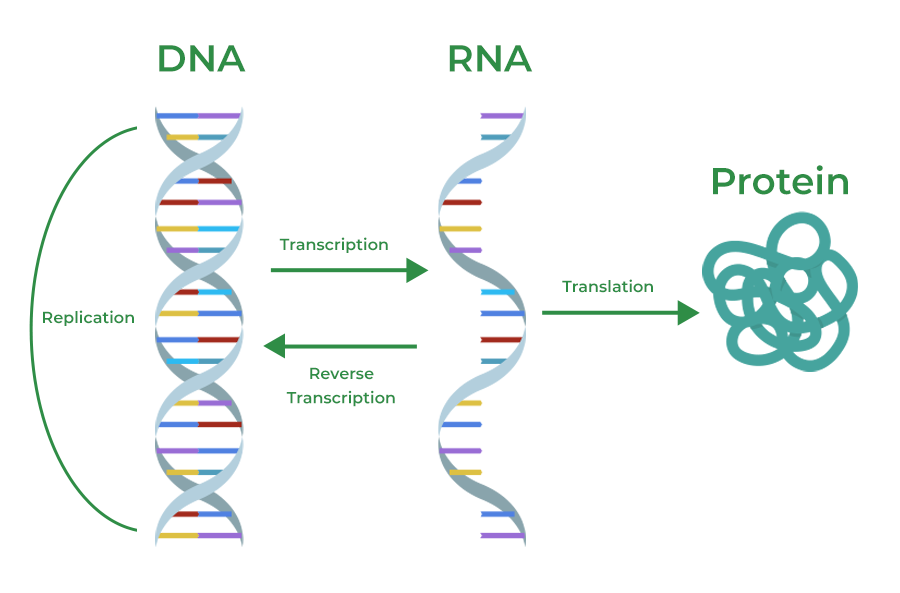
\includegraphics[width=\textwidth]{../../eukgen/images/dogma}
    \caption{Code Sonne von \url{https://www.geeksforgeeks.org/biology/central-dogma-steps-guide/}}
\end{figure}


\section{Rolle von Bakterien in der Genetik}
Bakterien sind so relevant, denn...

\begin{itemize}
    \item ...sie sind klein
    \item ...sie sind einfach zu kultivieren
    \item ...sie teilen sich sehr schnell
    \item ...sie sind genetisch gut zu bearbeiten
\end{itemize}

\defin{Genotyp}
\defin{Phänotyp}
\defin{Wildtyp}
\defin{Mutante}

\begin{bsp}
\textit{Xanthomonas campestris} \\
    Der \gls{Wildtyp} produziert Schleim (\gls{Phänotyp}) und in der \gls{Mutante} ist das Gen \textit{xanB}
verändert (\gls{Genotyp}), daher produziert sie keinen Schleim (\gls*{Phänotyp}).
\end{bsp}

\frage{avery}